\documentclass[12pt,letterpaper]{article}
\usepackage[margin=1in]{geometry}
\usepackage[T1]{fontenc}
\usepackage{lmodern}
\usepackage{amsmath,amssymb,booktabs,longtable,array,graphicx,setspace}
\usepackage[hidelinks]{hyperref}
\setstretch{1.85}
\setlength{\parskip}{0pt}
\setlength{\emergencystretch}{1em}
\setlength{\tabcolsep}{3pt}
\renewcommand{\thetable}{Web \arabic{table}}
\renewcommand{\thefigure}{Web \arabic{figure}}
\renewcommand{\thesection}{\Alph{section}}
\begin{document}
\begin{center}\textbf{Supplementary Material}\\Design and outcome-model estimability in doubly robust survival analysis: a breast cancer reanalysis\end{center}
This supplement and the main article are generated together from the supplied numerical outputs.
Clinical specification denotes the clinical adjustment set, covariate-conditional censoring and a 1095-day
post-landmark horizon unless stated otherwise. The older reference validation and calibration are separated
from the added Cox comparisons and independent stress scenarios.

\section{Estimators, assumptions and fixed preprocessing}
All expectations in this appendix refer to an eligible landmark population. Let $R=\min(T,\tau)$,
$Y=\min(\widetilde T,\tau)$, and $D$ indicate an observed death by $\tau$ or follow-up reaching $\tau$.
Write $m_a(X)=E(R\mid A=a,X)$ and $e(X)=\Pr(A=1\mid X)$.
Before stabilization, the complete-outcome AIPW contribution is
\begin{align*}
\psi(O)&=m_1(X)-m_0(X)\\
&\quad+\frac{AD}{e(X)G(Y^-\mid 1,X)}\{Y-m_1(X)\}\\
&\quad-\frac{(1-A)D}{\{1-e(X)\}G(Y^-\mid 0,X)}\{Y-m_0(X)\}.
\end{align*}
Under conditional independent censoring, $E(D\mid T,A,X)=G(R^-\mid A,X)$, with the stated
tie convention. For correct $G$, conditioning on $A,X$ gives
$E[D\{Y-m_a(X)\}/G(Y^-\mid a,X)\mid A=a,X]=m_a^0(X)-m_a(X)$,
where superscript 0 denotes the true conditional mean. Consequently,
\begin{align*}
E\{\psi(O)\mid X\}&=m_1(X)-m_0(X)\\
&\quad+\frac{e_0(X)}{e(X)}\{m_1^0(X)-m_1(X)\}\\
&\quad-\frac{1-e_0(X)}{1-e(X)}\{m_0^0(X)-m_0(X)\}.
\end{align*}
This recovers $m_1^0-m_0^0$ if $e=e_0$ or both outcome means are correct, conditional on correct $G$.
It does not provide robustness to arbitrary misspecification of $G$, and fixed weight truncation need not
retain this identity. It is not the full censoring-augmented efficient influence function.

Outcome regressions use complete cases weighted by $1/\widehat G$ inside treatment arms.
The propensity is ridge logistic; the censoring process uses ridge Cox with treatment strata and a
Breslow baseline. The unpenalized intercept is included in outcome/propensity parameter counts.
The adaptive penalty is $\lambda=\max\{1,p\max(1,10p/n)\}$ in the objective conventions in the code.
For AIPW propensity and outcome regressions, $p,n$ refer to the full input matrix and sample;
censoring fits compute their own training-sample penalty. Coefficients are trained on four of five folds.
Folds are stratified jointly by treatment and observed death within the horizon.

Clinical stage and TNM are ordinally encoded. Numeric missing values use full-cohort medians with
missing indicators. Sites with fewer than 20 patients in the landmark cohort are pooled; site coding is
fixed before restricting to a subgroup. Receptors defining TNBC are never imputed. The archived multimodal
matrix retains its previous processing; residual nonfinite entries are set to zero. These encodings and
clinical imputations are fixed for resampling. Within an AIPW input matrix, propensity/outcome scaling
also precedes fold splitting, whereas censoring-model scaling uses training observations. Bootstrap
refits therefore condition on the constructed feature matrix and do not reproduce original feature discovery.
No claim of fully nested model/feature selection is made.

Weighted KM clips propensity at 0.01/0.99; AIPW uses 0.02/0.98. Both floor $G$ at 0.05.
AIPW caps positive combined weights at the pooled 99th percentile, clips outcome means to $[0,\tau]$
and clips the contrast to $[-\tau,\tau]$. The Cox outcome comparator instead has one unpenalized treatment
coefficient, ridge-penalized standardized covariates, and a Breslow death-hazard baseline. Its arm-specific
survival predictions are averaged over the same observed covariate distribution and integrated exactly
between baseline-hazard knots. It does not use a separate censoring regression, relying on conditional
independent censoring and correct specification of the outcome model. Treatment contrast and hazard ratio
are distinct; only standardized RMST enters the comparison.

\section{Cohort audit and observed follow-up}
The starting frame is the supplied earlier cohort, not every patient ever enrolled in TCGA-BRCA.
The following ledger is sequential: each exclusion count refers to the preceding row's survivors.
Measured-receptor subgroup construction and original follow-up are shown in Web Figures 1--2.
The treatment-field comparison establishes discordance, not an externally validated error rate.

\begin{longtable}{p{4.3in}p{0.7in}p{0.8in}}
\caption{Day-90 analysis cohort ledger.}\\
\toprule
Rule & Excluded & Remaining \\
\midrule\endfirsthead
\toprule
Rule & Excluded & Remaining \\
\midrule\endhead
\bottomrule\endfoot
patients with an overall-survival record & -- & 1076 \\
missing survival data & 0 & 1076 \\
died or censored before day 90 (landmark not reached) & 57 & 1019 \\
received chemotherapy but start date missing (exposure undefined at the landmark) & 29 & 990 \\
chemotherapy start date before diagnosis (implausible) & 2 & 988 \\
\end{longtable}
\section{Complete effect estimates and proportional-hazards diagnostics}
Web Table 2 reports the original adjustment-set and horizon sensitivity estimates.
The new unadjusted KM and Cox clinical benchmarks and their bootstrap intervals are in main Table 1.
They use 2000 new patient bootstrap draws, paired with each other. Earlier KM intervals for a correction
ladder rung use their original seed, so Monte Carlo differences in endpoints do not imply different point estimates.
The complete proportional-hazards screens appear later in Web Table 11.

\begin{longtable}{p{1.6in}p{0.65in}p{1.1in}p{2.45in}}
\caption{All original adjusted RMST estimates. Intervals are patient-bootstrap percentile intervals.}\\
\toprule
Population/set & Horizon & Estimator & RMST (95\% interval) \\
\midrule\endfirsthead
\toprule
Population/set & Horizon & Estimator & RMST (95\% interval) \\
\midrule\endhead
\bottomrule\endfoot
TNBC / Clinical & 1095 & AIPW & 19.5 (-118.5, 179.7) \\
TNBC / Clinical & 1095 & Weighted KM & 55.0 (-24.4, 132.5) \\
TNBC / Existing & 1095 & AIPW & -5.4 (-113.3, 150.5) \\
TNBC / Existing & 1095 & Weighted KM & 28.6 (-37.9, 105.4) \\
TNBC / Union & 1095 & AIPW & 42.0 (-52.4, 133.2) \\
TNBC / Union & 1095 & Weighted KM & 45.8 (-27.7, 119.1) \\
TNBC / Clinical & 1825 & AIPW & 383.8 (107.5, 670.3) \\
TNBC / Clinical & 1825 & Weighted KM & 256.2 (31.9, 515.5) \\
TNBC / Existing & 1825 & AIPW & 13.0 (-449.3, 596.4) \\
TNBC / Existing & 1825 & Weighted KM & 121.1 (-74.9, 359.3) \\
TNBC / Union & 1825 & AIPW & 333.3 (35.5, 602.3) \\
TNBC / Union & 1825 & Weighted KM & 226.7 (9.5, 468.0) \\
Whole cohort / Clinical & 1095 & AIPW & -8.3 (-32.6, 84.7) \\
Whole cohort / Clinical & 1095 & Weighted KM & 37.8 (12.1, 71.6) \\
Whole cohort / Existing & 1095 & AIPW & -8.4 (-34.6, 53.3) \\
Whole cohort / Existing & 1095 & Weighted KM & 18.0 (-16.8, 60.3) \\
Whole cohort / Union & 1095 & AIPW & -20.5 (-30.8, 97.2) \\
Whole cohort / Union & 1095 & Weighted KM & 38.1 (8.8, 76.5) \\
Whole cohort / Clinical & 1825 & AIPW & 151.1 (34.7, 353.8) \\
Whole cohort / Clinical & 1825 & Weighted KM & 119.1 (44.8, 208.8) \\
Whole cohort / Existing & 1825 & AIPW & -42.7 (-130.7, 149.5) \\
Whole cohort / Existing & 1825 & Weighted KM & 108.7 (22.6, 226.6) \\
Whole cohort / Union & 1825 & AIPW & 134.3 (52.9, 350.4) \\
Whole cohort / Union & 1825 & Weighted KM & 124.5 (49.0, 219.1) \\
\end{longtable}
\begin{longtable}{p{1.0in}p{2.1in}p{0.8in}p{0.8in}p{0.9in}}
\caption{Estimator-specific balance. Values are absolute standardized mean differences (SMD). Treatment weights alone assess baseline balance; complete-outcome censoring weights define a different diagnostic.}\\
\toprule
Population & Weight definition & Mean SMD & Max SMD & No. $>0.1$ \\
\midrule\endfirsthead
\toprule
Population & Weight definition & Mean SMD & Max SMD & No. $>0.1$ \\
\midrule\endhead
\bottomrule\endfoot
TNBC & unweighted & 0.173 & 0.502 & 16 \\
TNBC & primary KM treatment weights & 0.113 & 0.379 & 11 \\
TNBC & AIPW treatment weights & 0.130 & 0.380 & 14 \\
Whole cohort & unweighted & 0.173 & 0.632 & 19 \\
Whole cohort & primary KM treatment weights & 0.051 & 0.196 & 4 \\
Whole cohort & AIPW treatment weights & 0.049 & 0.216 & 3 \\
\end{longtable}
\section{Censoring, horizon support and five-device stabilization}
Censoring diagnostics are evaluated at each complete case's restricted time. They differ between AIPW's
training-fold censoring fits and the primary estimator's full-sample fit. The combined-weight ESS values
reported in the article refer to capped AIPW complete-outcome residual weights; they are not an effective
sample size for the time-varying KM risk sets. Selected-horizon risk counts and estimator weight diagnostics
are supplied as CSV files. Sites with short follow-up motivate, but do not validate, conditional censoring models.

\begin{longtable}{p{1.7in}p{0.65in}p{2.25in}p{0.65in}p{0.55in}}
\caption{Original censoring-model sensitivity. Floor counts are complete cases with fitted censoring survival below 0.05.}\\
\toprule
Population/method & Model & RMST (95\% interval) & $G_{\min}$ & Floor \\
\midrule\endfirsthead
\toprule
Population/method & Model & RMST (95\% interval) & $G_{\min}$ & Floor \\
\midrule\endhead
\bottomrule\endfoot
TNBC / AIPW & Cox & 19.5 (-118.5, 179.7) & 0.027 & 2 \\
TNBC / AIPW & Arm KM & 75.5 (-42.6, 170.1) & 0.324 & 0 \\
TNBC / Weighted KM & Cox & 55.0 (-24.4, 132.5) & 0.078 & 0 \\
TNBC / Weighted KM & Arm KM & 52.1 (-27.7, 132.6) & 0.386 & 0 \\
Whole cohort / AIPW & Cox & -8.3 (-32.6, 84.7) & 0.002 & 7 \\
Whole cohort / AIPW & Arm KM & 28.4 (-15.5, 86.1) & 0.412 & 0 \\
Whole cohort / Weighted KM & Cox & 37.8 (12.1, 71.6) & 0.007 & 4 \\
Whole cohort / Weighted KM & Arm KM & 32.6 (10.2, 57.7) & 0.418 & 0 \\
\end{longtable}
\begin{longtable}{p{1.0in}p{3.0in}p{0.8in}p{1.0in}}
\caption{Updated stabilizer sensitivity, in RMST days. The joint relaxation now disables both prediction and contrast clipping, sets the propensity limits to 0.001/0.999 and censoring floor to 0.01, and removes the combined-weight cap. These remain near-untruncated rather than literally unbounded weights.}\\
\toprule
Population & Variant & AIPW & Weighted KM \\
\midrule\endfirsthead
\toprule
Population & Variant & AIPW & Weighted KM \\
\midrule\endhead
\bottomrule\endfoot
TNBC & specified & 19.5 & 55.0 \\
TNBC & propensity clip 0.01/0.99 & 19.5 & 55.0 \\
TNBC & propensity clip 0.001/0.999 & 19.5 & 55.0 \\
TNBC & censoring floor 0.02 & -52.0 & 55.0 \\
TNBC & censoring floor 0.10 & 69.4 & 55.6 \\
TNBC & combined weight cap 0.999 & 10.9 & 55.0 \\
TNBC & combined weight cap 0.95 & 100.2 & 55.0 \\
TNBC & outcome prediction clipping off & 19.8 & 55.0 \\
TNBC & contrast clipping off & 19.5 & 55.0 \\
TNBC & all five devices relaxed & -53.0 & 55.0 \\
TNBC & arm-only censoring & 75.5 & 52.1 \\
Whole cohort & specified & -8.3 & 37.8 \\
Whole cohort & propensity clip 0.01/0.99 & -8.3 & 37.8 \\
Whole cohort & propensity clip 0.001/0.999 & -8.3 & 37.8 \\
Whole cohort & censoring floor 0.02 & -12.2 & 42.9 \\
Whole cohort & censoring floor 0.10 & 13.2 & 36.4 \\
Whole cohort & combined weight cap 0.999 & -4.7 & 37.8 \\
Whole cohort & combined weight cap 0.95 & 19.4 & 37.8 \\
Whole cohort & outcome prediction clipping off & -9.1 & 37.8 \\
Whole cohort & contrast clipping off & -8.3 & 37.8 \\
Whole cohort & all five devices relaxed & -19.7 & 48.0 \\
Whole cohort & arm-only censoring & 28.4 & 32.6 \\
\end{longtable}
\section{Landmark, fold information and seed stability}
Changing to day 180 changes both eligibility and exposure status. It is a sensitivity analysis for a different
landmark population, not a bound on selection bias. The outcome effective degrees of freedom are computed
from the actual training-fit matrix and Cox-derived weights as
$\operatorname{tr}\{D(D^\top WD+P)^{-1}D^\top W\}$, where the intercept entry of $P$ is zero.
Fold-specific complete counts, dimension, penalty and effective degrees of freedom are supplied in
\texttt{20\_outcome\_fold\_df.csv}. Nominal rho counts use complete outcomes, not deaths alone.

\begin{longtable}{p{1.2in}p{0.8in}p{1.1in}p{2.7in}}
\caption{Day-180 landmark sensitivity at a 1095-day horizon.}\\
\toprule
Population & $n$/deaths & Estimator & RMST (95\% interval) \\
\midrule\endfirsthead
\toprule
Population & $n$/deaths & Estimator & RMST (95\% interval) \\
\midrule\endhead
\bottomrule\endfoot
TNBC & 133/16 & AIPW & 55.0 (-156.4, 277.2) \\
TNBC & 133/16 & Weighted KM & 83.3 (-40.6, 201.6) \\
Whole cohort & 971/69 & AIPW & 26.5 (-6.2, 123.1) \\
Whole cohort & 971/69 & Weighted KM & 44.5 (14.0, 78.7) \\
\end{longtable}
\begin{longtable}{p{1.85in}p{0.65in}p{1.0in}p{2.2in}}
\caption{Original six-seed repeat. This separates computational reproducibility from partition and simulation Monte Carlo variability.}\\
\toprule
Quantity & MC SD & Mean interval width & Interval reading \\
\midrule\endfirsthead
\toprule
Quantity & MC SD & Mean interval width & Interval reading \\
\midrule\endhead
\bottomrule\endfoot
TNBC IPCW-KM & 0.00 & 156.60 & interval spans zero \\
TNBC AIPW & 24.83 & 291.55 & interval spans zero \\
Whole cohort IPCW-KM & 0.00 & 59.89 & interval excludes zero \\
Whole cohort AIPW & 14.86 & 115.06 & interval spans zero \\
rho threshold (calibration) & 0.02 & 0.07 & triple-negative above, whole cohort below \\
\end{longtable}
\section{Original diagnostic calibration}
The 32-cell calibration uses four sample sizes (150, 300, 600, 1000), four covariate dimensions
(10, 25, 50, 75) and two baseline event-rate settings (0.12, 0.30). Each cell has 60 replicates.
Covariates are independent standard Gaussian. Treatment follows a logistic model with coefficients
$(0.7,-0.5,0.3)$ on the first three covariates and a centered linear predictor plus log odds for 0.6.
Survival is exponential with hazard $b\exp(0.5X_1+0.3X_2)0.65^A$, where
$b=-\log(1-r)/1095$. Censoring is exponential with mean $1.4\times1095$ and independent of covariates.
Adjustment sets are nested prefixes of size $\max(3,p/4)$, $\max(4,p/2)$ and $p$, with integer division.
All sets contain the assignment predictors. Sensitivity is the mean within-replicate range divided by
the full-set estimator's Monte Carlo sampling SD. The reported rho is averaged over replicates in a cell.
The log-linear fit and its crossing use 2000 bootstrap resamples of grid cells. These intervals reflect
variation across the selected cells and fit, not uncertainty over all possible data-generating regimes.
They also do not propagate every source of within-cell Monte Carlo uncertainty.
Penalty scales 0.3 and 3 use 30 replicates per cell; the specified scale uses 60.
The nested sets do not establish a lower bound on sensitivity under arbitrary real adjustment sets.

\begin{longtable}{p{1.9in}p{0.65in}p{1.0in}p{2.15in}}
\caption{Original warning-level sensitivities. The specified crossing is 0.50; the threshold is not an estimator-validity criterion.}\\
\toprule
Varied & Value & Threshold & 95\% cell-bootstrap \\
\midrule\endfirsthead
\toprule
Varied & Value & Threshold & 95\% cell-bootstrap \\
\midrule\endhead
\bottomrule\endfoot
Crossing & 0.25 & 0.11 & 0.09, 0.14 \\
Crossing & 0.50 & 0.31 & 0.28, 0.35 \\
Crossing & 0.75 & 0.88 & 0.74, 1.10 \\
Crossing & 1.00 & 2.47 & 1.84, 3.70 \\
Penalty multiplier & 0.3 & 0.22 & 0.19, 0.27 \\
Penalty multiplier & 1.0 & 0.31 & 0.28, 0.35 \\
Penalty multiplier & 3.0 & 1.32 & 0.70, 4.94 \\
\end{longtable}
\section{Validation against known truth and independent stress scenarios}
The original operating-point validation uses 500 replicates per scenario and 500 inner patient bootstrap
replicates. It simulates Gaussian covariates and exponential survival, logistic treatment and censoring
depending on a survival predictor. The input covariate counts are 25 and 28 before adding an intercept;
these approximate, rather than exactly match, the clinical outcome-model dimensions. Its event targets
and treated fractions are application-motivated. Empirical coverage cannot be assigned to the clinical
intervals merely because sample size and event counts are similar.

\begin{longtable}{p{1.85in}p{0.7in}p{0.7in}p{1.1in}p{1.1in}}
\caption{Original operating-point validation. SD is empirical estimate SD; SE is mean bootstrap SE. Coverage refers only to these simulated scenarios.}\\
\toprule
Scenario/method & Truth & Bias & SD/SE & Coverage \\
\midrule\endfirsthead
\toprule
Scenario/method & Truth & Bias & SD/SE & Coverage \\
\midrule\endhead
\bottomrule\endfoot
TNBC-like / AIPW & 44.2 & -1.4 & 65.1/63.4 & 95.0\% \\
TNBC-like / Weighted KM & 44.2 & -12.5 & 54.5/50.7 & 92.2\% \\
cohort-like / AIPW & 24.2 & 1.1 & 17.2/18.7 & 95.8\% \\
cohort-like / Weighted KM & 24.2 & -3.0 & 15.4/15.8 & 94.0\% \\
\end{longtable}
The independent stress study has six cells: $n=136,p=24$ or $n=988,p=27$, crossed with
three mechanisms. There are 200 replicates and 199 inner patient bootstraps per cell. New simulation seeds
are distinct from the original calibration. Gaussian scenarios use independent standard-normal covariates;
the nonlinear scenario uses independent $t_3/\sqrt{3}$ covariates. The default propensity is
$\operatorname{expit}(0.7X_1-0.5X_2+0.3X_3)$. The control death hazard is
$h_0=b\exp(0.5X_1+0.3X_2)$, and the censoring hazard is
$(\log 2/1100)\exp(0.5X_1+0.5X_3)$. Thus censoring depends on measured survival predictors.
The PH treatment hazard ratio is 0.65. The delayed-benefit scenario instead uses treatment hazard ratio
1.2 through day 365 and 0.45 thereafter; it violates a constant treatment hazard ratio in the Cox outcome model.

In the nonlinear heavy-tail scenario, add $0.6\mathbf{1}(X_1>1)$ to the propensity linear predictor,
replace the death predictor by $0.5X_1+0.5\sin(X_2)+0.3(X_3^2-1)$, and add $0.35(X_2^2-1)$
to the censoring predictor. Linear nuisance regressions are then misspecified. To keep the generated
hazards finite, death/censoring predictors are clipped to $[-4,4]$ and the propensity predictor to $[-20,20]$.
The baseline $b$ is calibrated by deterministic-seed numerical averaging over 30000 reference covariates
to expected observed deaths near 16 or 72. The exact fitted baseline constants are saved in
\texttt{21\_stress\_design.json}; achieved mean deaths are in the replicate and summary CSV files.

For hazards $h_1$ before $u=365$ and $h_2$ afterward, the restricted mean is
$(1-e^{-h_1u})/h_1+e^{-h_1u}(1-e^{-h_2(\tau-u)})/h_2$.
The treated-minus-control difference is averaged over each replicate's covariates to obtain its exact
conditional standardized truth. Four estimators are compared against this truth; the unadjusted KM
benchmark is expected to retain confounding. All estimators use their stated penalties and stabilization.
The AIPW fold seed is fixed within a replicate's bootstrap procedure. A replicate is evaluable for a method
only if its point estimate is finite and at least 95\% of its inner fits succeed. Failures are reported;
coverage is conditional on evaluability. Bias Monte Carlo SE is the SD of estimation errors divided by
the square root of evaluable replicates. Wilson intervals describe binomial Monte Carlo uncertainty in coverage.
RMSE is relative to each replicate's conditional truth. The full table also reports unadjusted KM;
the main coverage figure shows the three adjusted methods.

\begin{longtable}{p{2.0in}p{1.0in}p{0.6in}p{1.7in}p{0.55in}}
\caption{Independent stress validation. Bias is accompanied by its Monte Carlo SE. Coverage includes a 95\% Wilson Monte Carlo interval. Failures are out of 200 replicates per cell and estimator; all individual results are supplied.}\\
\toprule
Scenario / $n$ / method & Bias (MC SE) & RMSE & Coverage (MC interval) & Failed \\
\midrule\endfirsthead
\toprule
Scenario / $n$ / method & Bias (MC SE) & RMSE & Coverage (MC interval) & Failed \\
\midrule\endhead
\bottomrule\endfoot
PH / conditional censoring / 136 / AIPW & 3.4 (3.6) & 50.8 & 97.5 (94.3, 98.9) & 0 \\
PH / conditional censoring / 136 / Cox RMST & -13.3 (2.6) & 39.1 & 91.5 (86.8, 94.6) & 0 \\
PH / conditional censoring / 136 / Weighted KM & -14.0 (3.1) & 46.5 & 93.0 (88.6, 95.8) & 0 \\
PH / conditional censoring / 136 / Unadjusted KM & -19.5 (3.1) & 48.3 & 95.0 (91.0, 97.3) & 0 \\
PH / conditional censoring / 988 / AIPW & 5.2 (1.5) & 21.5 & 94.0 (89.8, 96.5) & 0 \\
PH / conditional censoring / 988 / Cox RMST & 0.2 (0.9) & 12.5 & 92.0 (87.4, 95.0) & 0 \\
PH / conditional censoring / 988 / Weighted KM & -0.7 (1.3) & 18.6 & 91.5 (86.8, 94.6) & 0 \\
PH / conditional censoring / 988 / Unadjusted KM & -8.6 (1.0) & 17.1 & 85.5 (80.0, 89.7) & 0 \\
Delayed benefit / 136 / AIPW & 6.2 (4.2) & 59.8 & 97.0 (93.6, 98.6) & 0 \\
Delayed benefit / 136 / Cox RMST & 14.7 (2.7) & 40.7 & 91.0 (86.2, 94.2) & 1 \\
Delayed benefit / 136 / Weighted KM & -13.5 (3.5) & 50.8 & 92.5 (88.0, 95.4) & 0 \\
Delayed benefit / 136 / Unadjusted KM & -16.4 (3.4) & 50.8 & 93.5 (89.2, 96.2) & 0 \\
Delayed benefit / 988 / AIPW & 4.8 (1.5) & 21.0 & 93.0 (88.6, 95.8) & 0 \\
Delayed benefit / 988 / Cox RMST & 19.2 (0.8) & 22.5 & 63.5 (56.6, 69.9) & 0 \\
Delayed benefit / 988 / Weighted KM & -0.7 (1.3) & 18.1 & 92.0 (87.4, 95.0) & 0 \\
Delayed benefit / 988 / Unadjusted KM & -8.2 (1.1) & 17.3 & 90.5 (85.6, 93.8) & 0 \\
Nonlinear / heavy tail / 136 / AIPW & 1.2 (3.7) & 51.7 & 98.5 (95.7, 99.5) & 0 \\
Nonlinear / heavy tail / 136 / Cox RMST & -5.7 (2.5) & 36.1 & 93.0 (88.6, 95.8) & 0 \\
Nonlinear / heavy tail / 136 / Weighted KM & -5.5 (3.2) & 46.1 & 94.5 (90.4, 96.9) & 0 \\
Nonlinear / heavy tail / 136 / Unadjusted KM & -5.3 (3.2) & 45.0 & 95.5 (91.7, 97.6) & 0 \\
Nonlinear / heavy tail / 988 / AIPW & -2.6 (1.3) & 18.9 & 93.0 (88.6, 95.8) & 0 \\
Nonlinear / heavy tail / 988 / Cox RMST & -0.4 (0.8) & 11.0 & 92.5 (88.0, 95.4) & 0 \\
Nonlinear / heavy tail / 988 / Weighted KM & -3.5 (1.4) & 20.3 & 89.5 (84.5, 93.0) & 0 \\
Nonlinear / heavy tail / 988 / Unadjusted KM & -5.7 (1.1) & 16.5 & 88.5 (83.3, 92.2) & 0 \\
\end{longtable}
Schoenfeld rank-time screens use lifelines Efron-tie reference refits for the death and censoring
processes. Penalties are converted to the code's scale, the treatment coefficient is unpenalized in the
death model, and censoring is stratified by treatment. Holm adjustment is within each model over covariates.
These exploratory checks use penalized fits, are not exact finite-sample tests, and cannot verify independent
censoring. They are reported as potential model-fit concerns, not automatic model acceptance/rejection.

\begin{longtable}{p{1.55in}p{2.25in}p{0.9in}p{1.1in}}
\caption{Complete proportional-hazards screens. Raw and within-model Holm-adjusted p-values; Efron reference refits.}\\
\toprule
Population/process & Covariate & Raw $p$ & Holm $p$ \\
\midrule\endfirsthead
\toprule
Population/process & Covariate & Raw $p$ & Holm $p$ \\
\midrule\endhead
\bottomrule\endfoot
TNBC / death & age & 0.2747 & 1 \\
TNBC / death & chemotherapy\_by\_landmark & 0.215 & 1 \\
TNBC / death & m\_stage & 0.9013 & 1 \\
TNBC / death & m\_stage\_missing & 0.3966 & 1 \\
TNBC / death & n\_stage & 0.1174 & 1 \\
TNBC / death & site\_A2 & 0.9742 & 1 \\
TNBC / death & site\_A7 & 0.8577 & 1 \\
TNBC / death & site\_A8 & 0.7965 & 1 \\
TNBC / death & site\_AC & 0.7188 & 1 \\
TNBC / death & site\_AO & 0.9912 & 1 \\
TNBC / death & site\_AR & 0.8034 & 1 \\
TNBC / death & site\_B6 & 0.633 & 1 \\
TNBC / death & site\_BH & 0.9795 & 1 \\
TNBC / death & site\_C8 & 0.6166 & 1 \\
TNBC / death & site\_D8 & 0.8823 & 1 \\
TNBC / death & site\_E2 & 0.8408 & 1 \\
TNBC / death & site\_E9 & 0.9545 & 1 \\
TNBC / death & site\_EW & 0.7372 & 1 \\
TNBC / death & site\_GM & 0.721 & 1 \\
TNBC / death & site\_OL & 0.7565 & 1 \\
TNBC / death & site\_OTHER & 0.9205 & 1 \\
TNBC / death & stage & 0.3674 & 1 \\
TNBC / death & stage\_missing & 0.8821 & 1 \\
TNBC / death & t\_stage & 0.4404 & 1 \\
TNBC / death & year\_dx & 0.4579 & 1 \\
TNBC / censoring & age & 0.5401 & 1 \\
TNBC / censoring & m\_stage & 0.4205 & 1 \\
TNBC / censoring & m\_stage\_missing & 0.5916 & 1 \\
TNBC / censoring & n\_stage & 0.6095 & 1 \\
TNBC / censoring & site\_A2 & 0.8813 & 1 \\
TNBC / censoring & site\_A7 & 0.9195 & 1 \\
TNBC / censoring & site\_A8 & 0.679 & 1 \\
TNBC / censoring & site\_AC & 0.7895 & 1 \\
TNBC / censoring & site\_AO & 0.3824 & 1 \\
TNBC / censoring & site\_AR & 0.3135 & 1 \\
TNBC / censoring & site\_B6 & 0.3775 & 1 \\
TNBC / censoring & site\_BH & 0.8489 & 1 \\
TNBC / censoring & site\_C8 & 0.9864 & 1 \\
TNBC / censoring & site\_D8 & 0.7598 & 1 \\
TNBC / censoring & site\_E2 & 0.6786 & 1 \\
TNBC / censoring & site\_E9 & 0.7904 & 1 \\
TNBC / censoring & site\_EW & 0.7165 & 1 \\
TNBC / censoring & site\_GM & 0.4778 & 1 \\
TNBC / censoring & site\_OL & 0.9207 & 1 \\
TNBC / censoring & site\_OTHER & 0.9551 & 1 \\
TNBC / censoring & stage & 0.8732 & 1 \\
TNBC / censoring & stage\_missing & 0.6672 & 1 \\
TNBC / censoring & t\_stage & 0.7585 & 1 \\
TNBC / censoring & year\_dx & 0.9507 & 1 \\
Whole cohort / death & age & 0.2479 & 1 \\
Whole cohort / death & chemotherapy\_by\_landmark & 0.9621 & 1 \\
Whole cohort / death & m\_stage & 0.7122 & 1 \\
Whole cohort / death & m\_stage\_missing & 0.2252 & 1 \\
Whole cohort / death & n\_stage & 0.8597 & 1 \\
Whole cohort / death & n\_stage\_missing & 0.9364 & 1 \\
Whole cohort / death & site\_A2 & 0.8134 & 1 \\
Whole cohort / death & site\_A7 & 0.7927 & 1 \\
Whole cohort / death & site\_A8 & 0.3653 & 1 \\
Whole cohort / death & site\_AC & 0.4389 & 1 \\
Whole cohort / death & site\_AO & 0.3319 & 1 \\
Whole cohort / death & site\_AR & 0.09758 & 1 \\
Whole cohort / death & site\_B6 & 0.2263 & 1 \\
Whole cohort / death & site\_BH & 0.3245 & 1 \\
Whole cohort / death & site\_C8 & 0.5864 & 1 \\
Whole cohort / death & site\_D8 & 0.9438 & 1 \\
Whole cohort / death & site\_E2 & 0.7668 & 1 \\
Whole cohort / death & site\_E9 & 0.2856 & 1 \\
Whole cohort / death & site\_EW & 0.8112 & 1 \\
Whole cohort / death & site\_GM & 0.3529 & 1 \\
Whole cohort / death & site\_OL & 0.6205 & 1 \\
Whole cohort / death & site\_OTHER & 0.2142 & 1 \\
Whole cohort / death & stage & 0.4257 & 1 \\
Whole cohort / death & stage\_missing & 0.6634 & 1 \\
Whole cohort / death & t\_stage & 0.1907 & 1 \\
Whole cohort / death & t\_stage\_missing & 0.7374 & 1 \\
Whole cohort / death & year\_dx & 0.08829 & 1 \\
Whole cohort / death & year\_dx\_missing & 0.1955 & 1 \\
Whole cohort / censoring & age & 0.3094 & 1 \\
Whole cohort / censoring & m\_stage & 0.8586 & 1 \\
Whole cohort / censoring & m\_stage\_missing & 0.04202 & 1 \\
Whole cohort / censoring & n\_stage & 0.9458 & 1 \\
Whole cohort / censoring & n\_stage\_missing & 0.599 & 1 \\
Whole cohort / censoring & site\_A2 & 0.8195 & 1 \\
Whole cohort / censoring & site\_A7 & 0.5087 & 1 \\
Whole cohort / censoring & site\_A8 & 0.1479 & 1 \\
Whole cohort / censoring & site\_AC & 0.3223 & 1 \\
Whole cohort / censoring & site\_AO & 0.1056 & 1 \\
Whole cohort / censoring & site\_AR & 0.6939 & 1 \\
Whole cohort / censoring & site\_B6 & 0.9485 & 1 \\
Whole cohort / censoring & site\_BH & 0.4581 & 1 \\
Whole cohort / censoring & site\_C8 & 0.4829 & 1 \\
Whole cohort / censoring & site\_D8 & 0.637 & 1 \\
Whole cohort / censoring & site\_E2 & 0.9571 & 1 \\
Whole cohort / censoring & site\_E9 & 0.966 & 1 \\
Whole cohort / censoring & site\_EW & 0.6094 & 1 \\
Whole cohort / censoring & site\_GM & 0.6969 & 1 \\
Whole cohort / censoring & site\_OL & 0.9758 & 1 \\
Whole cohort / censoring & site\_OTHER & 0.01529 & 0.3975 \\
Whole cohort / censoring & stage & 0.9606 & 1 \\
Whole cohort / censoring & stage\_missing & 0.7019 & 1 \\
Whole cohort / censoring & t\_stage & 0.8791 & 1 \\
Whole cohort / censoring & t\_stage\_missing & 0.7006 & 1 \\
Whole cohort / censoring & year\_dx & 8.414e-05 & 0.002272 \\
Whole cohort / censoring & year\_dx\_missing & 0.7684 & 1 \\
\end{longtable}
\section{Exploratory heterogeneity and scope of validation}
The earlier analysis gated heterogeneity at 50 deaths, a convention rather than a guarantee of usable
power. Only whole-cohort estimates are retained here. Their AIPW scores are cross-fitted for nuisance
estimation, but the later linear ranking was fitted and evaluated on the same cohort. The old subgroup,
BLP and RATE intervals resampled already computed scores rather than the full estimation procedure.
They are therefore omitted from this submission's heterogeneity table. This avoids presenting conditional
fixed-score intervals as if they reflected all nuisance, ranking and selection uncertainty.
The following estimates are descriptive only and do not establish targeting ability or effect modification.
Confirmatory RATE evaluation would require an independently learned ranking or an appropriate additional
cross-fitting scheme; nominal significance of the old interval is not used as evidence.

For context, the earlier approximate minimum-detectable subgroup differences are TNBC: 279.2 days; Whole cohort: 82.2 days. These use $2(z_{0.975}+z_{0.80})s/\sqrt{nq(1-q)}$, where $q$ is the treated fraction and $s$ is the restricted-time SD among complete cases. They are rough complete-data calculations, not power calculations for the weighted survival estimator, censoring or a prespecified interaction test. The 50-death gate and this approximation do not establish adequate power.
\begin{longtable}{p{1.45in}p{2.55in}p{0.6in}p{1.15in}}
\caption{Whole-cohort descriptive heterogeneity summaries. No confirmatory intervals are assigned. BLP denotes best linear projection; AUTOC is an in-sample ranking summary.}\\
\toprule
Analysis & Term & $n$ & Estimate, days \\
\midrule\endfirsthead
\toprule
Analysis & Term & $n$ & Estimate, days \\
\midrule\endhead
\bottomrule\endfoot
group effect & age $<$ 50 & 272 & -8.6 \\
group effect & age $\ge$ 50 & 716 & -8.2 \\
group effect & node negative (N0) & 467 & -31.2 \\
group effect & node positive (N1-3) & 506 & 46.5 \\
group effect & stage I-II & 733 & -31.2 \\
group effect & stage III-IV & 233 & 66.8 \\
BLP of CATE & intercept (ATE) & 988 & -8.3 \\
BLP of CATE & age (centred) & 988 & 2.1 \\
BLP of CATE & node positive & 988 & 100.7 \\
BLP of CATE & stage III-IV & 988 & 40.8 \\
CATE calibration & quintile 1 & 198 & -6.6 \\
CATE calibration & quintile 2 & 200 & -84.9 \\
CATE calibration & quintile 3 & 199 & -65.3 \\
CATE calibration & quintile 4 & 203 & -31.2 \\
CATE calibration & quintile 5 & 188 & 156.3 \\
RATE (AUTOC) & AUTOC & 988 & 79.4 \\
\end{longtable}
Classification and clustering metrics do not evaluate the RMST contrast. Biological gene-set
enrichment would require a defined gene universe and molecular-selection target; no new signature is
proposed here. Statistical validation instead examines the specified estimators against known RMST truth,
alongside support, fit and sensitivity diagnostics. The related prognostic study addresses transport and
incremental predictive utility separately.

\section{Reproducibility, software and files}
The code-and-data supplement provides the clinical and derived inputs, generated CSV outputs, software
requirements, seed and source hashes, and a single pipeline entry point. The analysis uses NumPy/Pandas;
figures use Matplotlib, and the comparator cross-checks and PH screens use lifelines/SciPy. LaTeX compilation
is included in the documented build command. The original Kaplan--Meier, RMST and Cox-censoring cross-checks
are retained in \texttt{15\_lifelines\_crosscheck.csv}. The new Cox RMST implementation is independently
checked against lifelines on untied unpenalized data, under treatment relabeling, constant-column addition
and feasible-range constraints. Agreement of a numerical component does not validate a clinical model.

The supplied raw clinical exports and derived survival/feature tables suffice for the analyses in this paper.
The original raw omics matrices and Xena source export are not reconstructed. Input SHA-256 digests and
the distinction between supplied inputs and upstream provenance are documented in the plain-text README.
The bootstrap and simulation replication counts are recorded in their output tables. Reduced smoke runs
write into a separate directory and are never used to generate the submission PDFs.

\section{Related work, archived implementation and scope}
The earlier covariate list was intended as an input to a published feature-selection framework's downstream
analysis. The archived implementation accepted a feature-list argument but substituted a univariate
penalized-Cox screen. The source location is in the feature-extraction tree. This observation concerns that
archived routine; it does not establish which routine generated the published framework's results, and
no claim is made that those published results are affected or unaffected. The archived source file is
available from the authors on request. The feature-selection framework itself
is not re-evaluated in the current manuscript.

Two related manuscripts are under review. Auditing Treatment Sequencing in Landmark Analyses of Treatment Initiation: An Empirically Anchored Simulation and Breast Cancer Application (submitted to Statistical Methods in Medical Research) audits treatment sequencing in landmark analyses of treatment initiation. Separating Assayability, Stability, and Incremental Utility in Cross-Cohort Multi-Omics Prognostic Evaluation: A Reproducible TCGA-METABRIC Framework (under consideration at Network Modeling Analysis in Health Informatics and Bioinformatics) studies cross-cohort prognostic evaluation. The present manuscript instead estimates chemotherapy landmark contrasts and studies nuisance-model information and estimator sensitivity. The manuscripts share TCGA breast cancer data and aspects of the earlier cohort construction; neither is presented as independent validation of the current treatment contrast.

Generative AI assistance with coding, documentation and editorial preparation is disclosed in the article
and cover letter. No grant supported this reanalysis. All authors must approve the final manuscript and
contributor statements before submission.

\clearpage\begin{figure}[p]\setstretch{1.85}\centering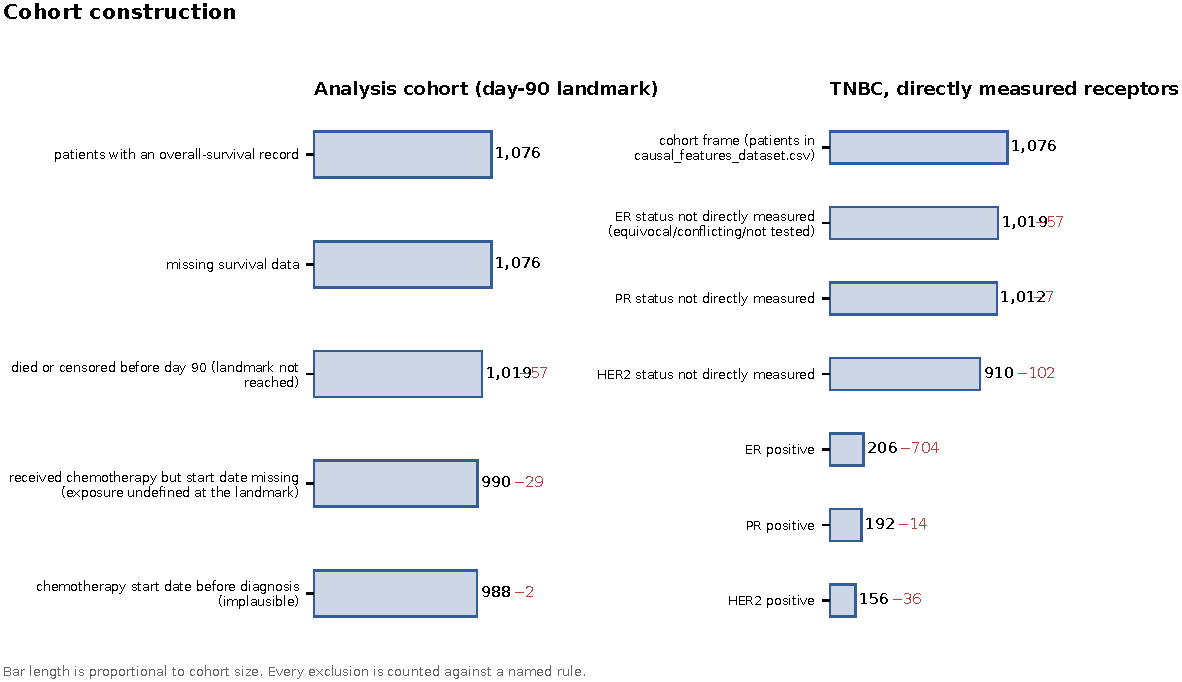
\includegraphics[width=\textwidth,height=0.70\textheight,keepaspectratio]{figures/fig1_cohort_flow.pdf}\caption{Cohort construction and measured TNBC definition. Each exclusion is counted.}\end{figure}
\clearpage\begin{figure}[p]\setstretch{1.85}\centering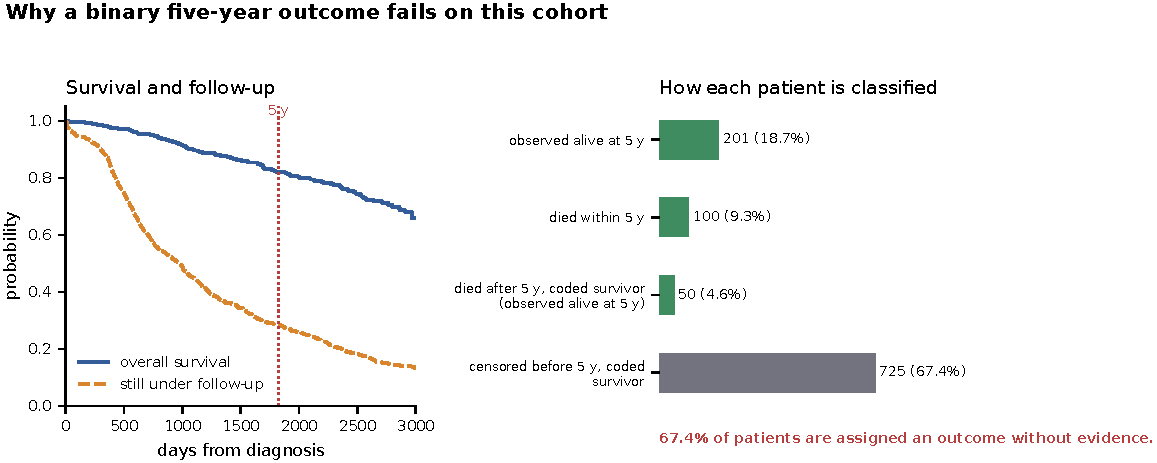
\includegraphics[width=\textwidth,height=0.70\textheight,keepaspectratio]{figures/fig2_censoring.pdf}\caption{Original-cohort survival and follow-up, and ascertainment of the five-year binary endpoint.}\end{figure}
\clearpage\begin{figure}[p]\setstretch{1.85}\centering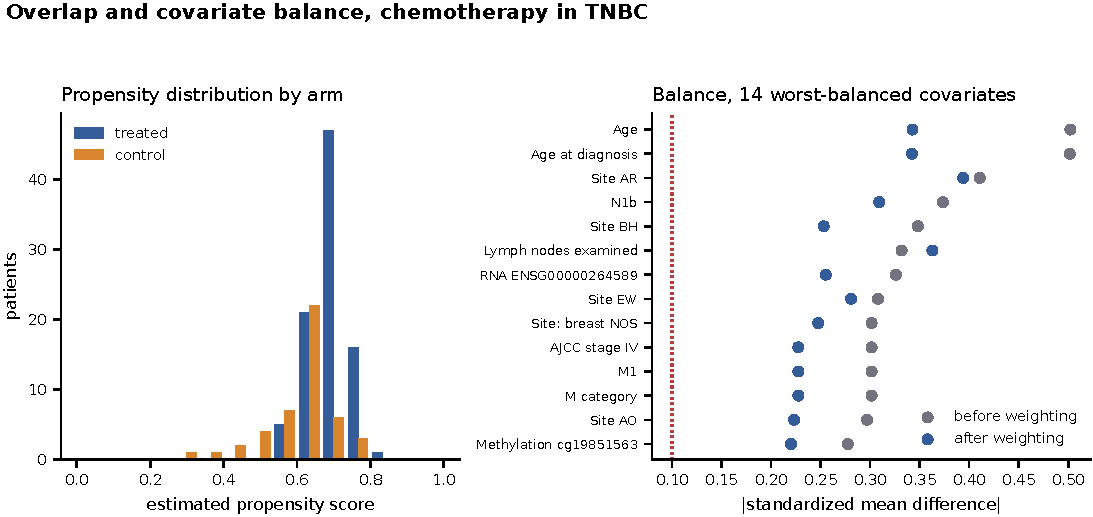
\includegraphics[width=\textwidth,height=0.70\textheight,keepaspectratio]{figures/fig4_overlap_balance.pdf}\caption{Earlier union-set TNBC propensity and balance display, retained as a sensitivity diagnostic. Main-text clinical-primary balance is separately recomputed from the primary estimator weights.}\end{figure}
\clearpage\begin{figure}[p]\setstretch{1.85}\centering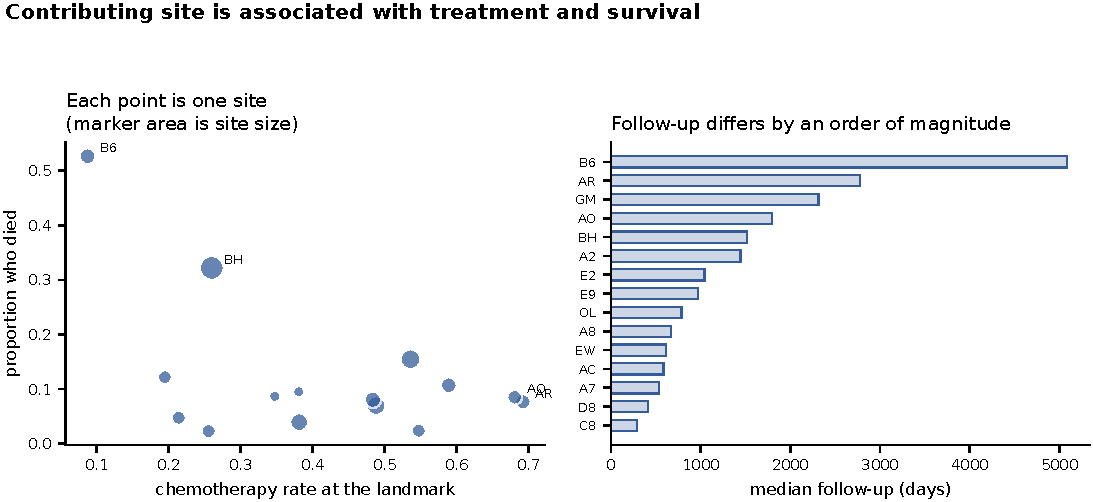
\includegraphics[width=\textwidth,height=0.70\textheight,keepaspectratio]{figures/fig5_site_confounding.pdf}\caption{Site-level treatment and follow-up summaries. Association alone does not establish that site is a confounder.}\end{figure}
\end{document}